\chapter{Other applications and future work}
\label{chap:applications}

Both \mx and \varan are designed as flexible frameworks which could be extended
tp support a variety of application scenarios involving NVX systems. In this
chapter, we discuss three such scenarios: transparent failover live
sanitization (\S\ref{sec:sanitization}), record-replay
(\S\ref{sec:record_replay}), and security honeypots (\S\ref{sec:honeypot}). We
also present other possible future extensions to both \mx and \varan.

% \subsubsection{Regression Testing}
% \label{sec:testing}

% One of the most obvious applications of \varan framework is regression testing.
% Developers often made various assumption about their programs. When working on
% a new version, regression testing is often used to ensure that these
% assumptions still hold even in the new version. Unfortunately, testing is not
% an exhaustive technique and since regression tests are often written by the
% same developers as the software itself, there is a high probability that some
% violations will be violated leading to security bugs~\todo{Give concrete
% examples.}.

% Executing the regression suite under \varan while running both versions in
% parallel (possibly even more) might help to reveal the subtle differences,
% otherwise undetected by the tests. Our current prototype can be instructed to
% stop the application when a divergence in the event stream is discovered
% providing a detailed information of the difference (\eg system call and its
% arguments). \varan may also attempt to continue execution performing different
% system calls. However, this may not always be possible (\eg in case of network
% communication), see discussion in \ref{sec:patternmatching} for more details.

\section{Live sanitization}
\label{sec:sanitization}

\begin{figure}[t]
  \begin{center}
    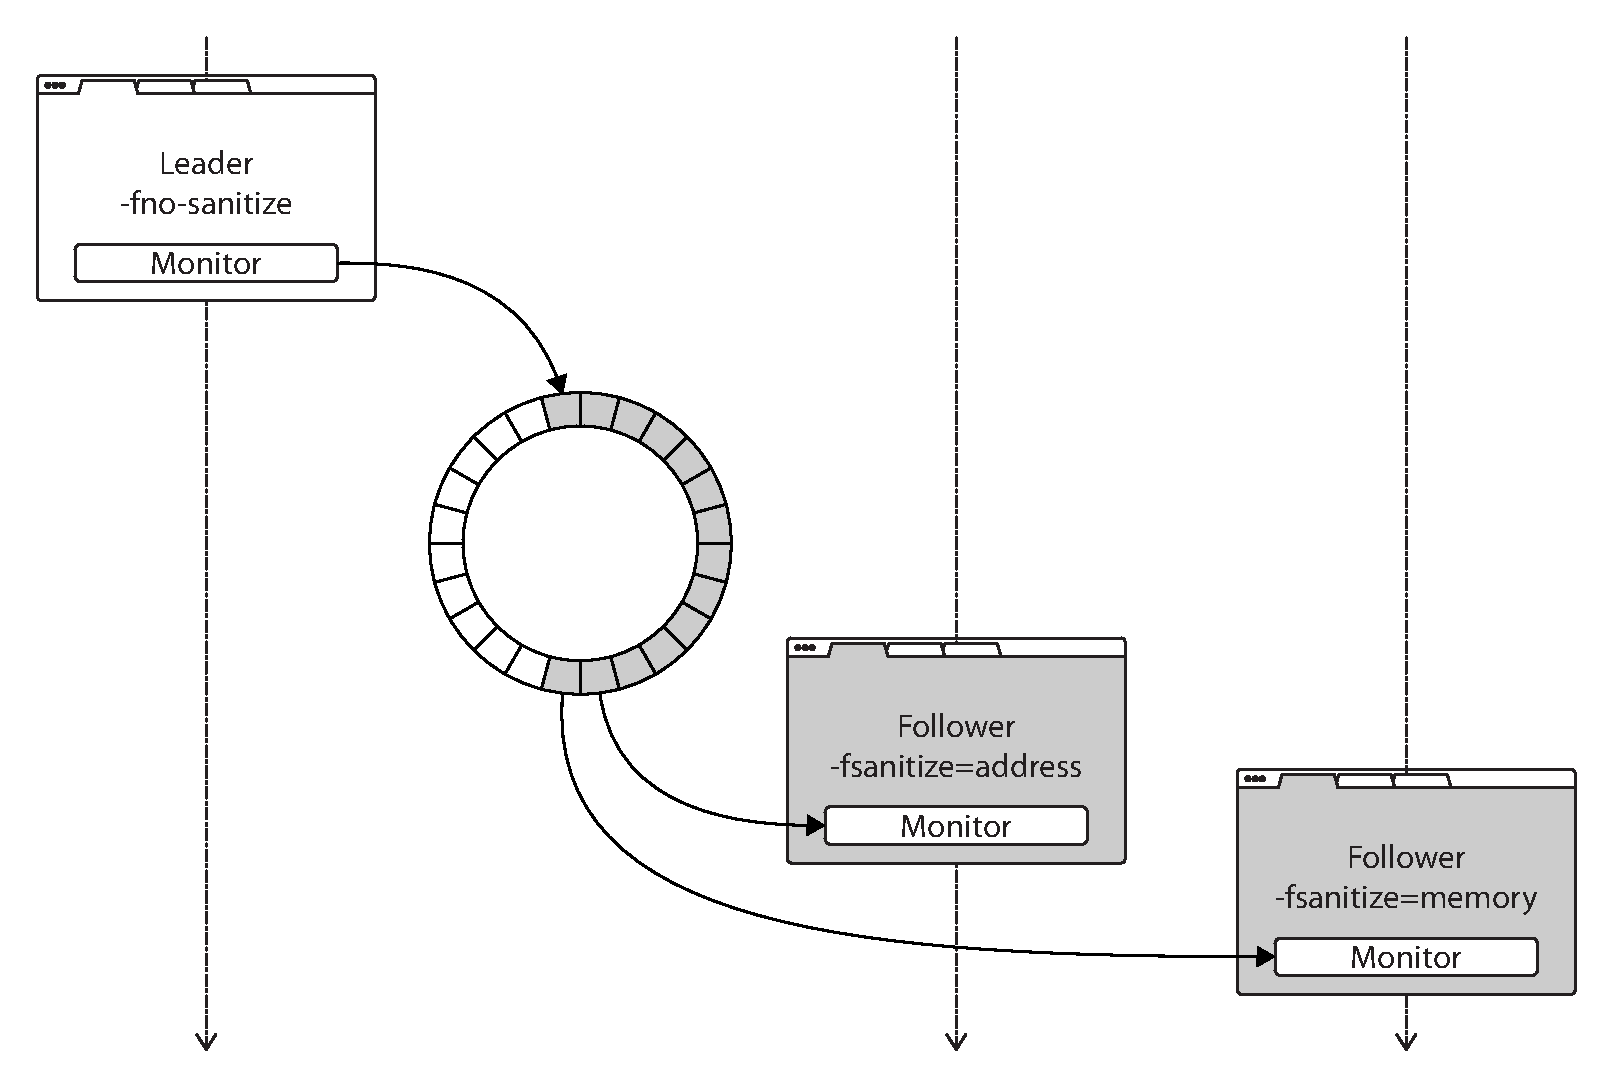
\includegraphics[width=0.75\columnwidth]{applications/figures/live-sanitization}
    \caption{The use of event-streaming architecture for live sanitization.}
    \label{fig:live-sanitization}
  \end{center}
\end{figure}

Sanitization is one of the most effective testing techniques for revealing
low-level bugs such as uninitialized pointer dereferences and use-after-free
errors.  Both Clang and GNU C Compiler now include a set of
sanitizers---AddressSanitizer (ASan), MemorySanitizer (MSan), ThreadSanitizer
(TSan)---which can be used to statically instrument the code with various
checks.  Unfortunately, these checks introduce extra overhead (\eg $~2\times$
for ASan, $~3\times$ for MSan and $~5$-$15\times$ for TSan).  which is why
these sanitizers are typically only used in offline testing. However, during
testing developers only use a limited set of inputs which might not reveal all
bugs.

One possible solution is to record execution traces during deployment and then
replay them in a testing environment with sanitization enabled. However, this
approach is unlikely to work in practice for several reasons. First, since we
do not know in advance which traces are potentially interesting (\eg trigger
sanitization checks) and which are not, we have to potentially collect and
replay a huge number of execution traces. Even with some form of deduplication,
this is usually impractical. Second, for long-running applications such as
servers, the log size will quickly grow to a large size. Third, many customers
will refuse to share the logs from their production deployment.

With \varan, we can perform live sanitization by running the native unsanitized
version as the leader, with sanitized versions as followers, as shown in
Figure~\ref{fig:live-sanitization}.  While sanitization itself introduces a
performance overhead, since followers do not need to execute any I/O operations
and merely replay them, they can often keep up with the leader, allowing users
to run sanitized versions in production without introducing any significant
overhead.

To demonstrate this, we build revision \lstinline`7f77235` of \redis twice:
once with Clang without any sanitization, once with ASan enabled.  We then ran
both versions in parallel using \varan and used the same benchmark with the
same settings as for our performance evaluation (\S\ref{sec:c10k}). As
expected, we have not measured any additional slowdown in the leader compared
to the scenario with two non-sanitized versions being run in parallel. To get a
better insight into the effect of running the sanitized version with \varan, we
have measured the median length of the log, \ie the distance between the leader
and the follower. With sanitization, this length increases from
\redisNoSanitizationMedianLength to \redisSanitizationMedianLength, which does
not impose any problems.

\section{Record-Replay}
\label{sec:record_replay}

Although \varan shares similarities with record-replay systems, there are
significant differences; in particular, the log is of fixed size and
only kept in-memory.  However, it is possible to easily extend \varan to
provide full record-replay capabilities by implementing two artificial
clients:
\begin{inparaenum}[(i)]
\item one acting as a \emph{follower} whose only goal is to write the
  content of the ring buffer to persistent storage, and
\item one acting as a \emph{leader}, reading the content of the log
  from the persistent storage and publishing events into the ring
  buffer for consumption by other clients.
\end{inparaenum}

Compared to some of the previous record-replay systems, \varan has a
number of advantages. First, decoupling the logic responsible for
reading/writing the log from the actual application into a separate
process allows the application to run at nearly full speed and utilize
the multiple cores available in modern CPUs.  Second, since \varan was
designed to run multiple instances at the same time, we can replay
multiple versions at once, \eg to determine which versions of the
application from a given range are susceptible to a crash reported by
the user.

We have implemented a simple prototype of the two aforementioned
clients on top of \varan and compared its performance against
\scribe~\cite{scribe}, a state-of-the-art record-replay system
implemented in the kernel.  Unfortunately, because \scribe is
implemented in the kernel and is only maintained for an old 32-bit
Linux kernel (2.6.35), we had to run our experiments inside a virtual
machine (kindly provided to us by \scribe's authors, as the source tree
was broken at the time of our experiments). 
%% This experience clearly shows one of the main disadvantages of
%% kernel-level frameworks---the difficulty of maintaining the code base.
To allow for a more faithful comparison, we ran \varan inside the same
virtual machine.

We used \redis as a benchmark, running the same workload as before,
and configured both systems to record the execution to persistent
storage.  We recorded an overhead of \redisRROvhScribe for
\scribe,\footnote{The overhead we measured for \scribe is higher than
  the overhead reported in~\cite{scribe}; however, note that the original
  work used less aggressive benchmarks such as \httpd.  The use of a
  virtual machine also affected the result.}  compared to
\redisRROvhNx for \varan.
%(but remember that we ran it inside a virtual machine)

% Despite being implemented in the kernel, \scribe
% performed worse than \varan on our \redis experiments: the overhead
% introduced by \scribe was \redisRROvhScribe, compared to only
% \redisRROvhNx for \varan.



\section{Security honeypot}
\label{sec:honeypot}

The ability to perform parallel multi-version execution could be also used to
deploy high-interaction honeypots that can offer a detailed account of the
attackers' activities. These honeypots could run vulnerable versions of
security critical services, and compare their behaviour, in real time, against
that of a known secure version.  Any divergence detected could be resolved in
favour of the secure version and logged for further analysis.  This would
provide a fine-grained understanding of the anatomy of an attack, which is
typically not possible with today's honeypot deployments. The construction
of such a honeypot system using an existing multi-variant execution
environment has been already proposed in the past~\cite{jackson10} but,
to our knowledge, no implementation of such mechanism exists.
%The use of multi-variant execution to construct such honeypot systems has been
%already proposed in the past~\cite{jackson10}. However, to our knowledge, no
%general-purpose implementation of such mechanism exists.

We have implemented this security mechanism in a simple prototype system based
on top of \varan. This system runs two variants of an
application---\emph{public} and \emph{private}---in lockstep and monitors their
behavior. A monitor synchronizes the execution of the two variants and grants
or denies access to operating system resources. Any divergence in the variant
behavior might be a sign of an ongoing attack. While this prototype reuses
large part of the \varan's codebase, namely the preloader, the monitor and the
system call interception mechanism, there are several important differences.

In regular multi-variant or multi-version application, all versions run on the
same machine in the same action scope under the same security restrictions.
However, in the honeypot system, each variant has a different action scope and
different access to operating system resources such file system and network.

For example, consider a web service running on top of the multi-variant
honeypot (MVH). A public variant is granted and access to network resources
while the private variant can only access the file system. Every request
received by the public variant is forwarded to the private variant through the
monitor, and after being processed, the result is sent back to the public
version. When the public version is compromised due to an existing (potentially
unknown) vulnerability, it might issue and additional system calls in an
attempt to access local resources; this will result in a divergence which will
be detected and recorded by the monitor. The monitor will also close the
connection to the private variant to protect any critical resources.

\begin{figure}[t]
  \begin{center}
    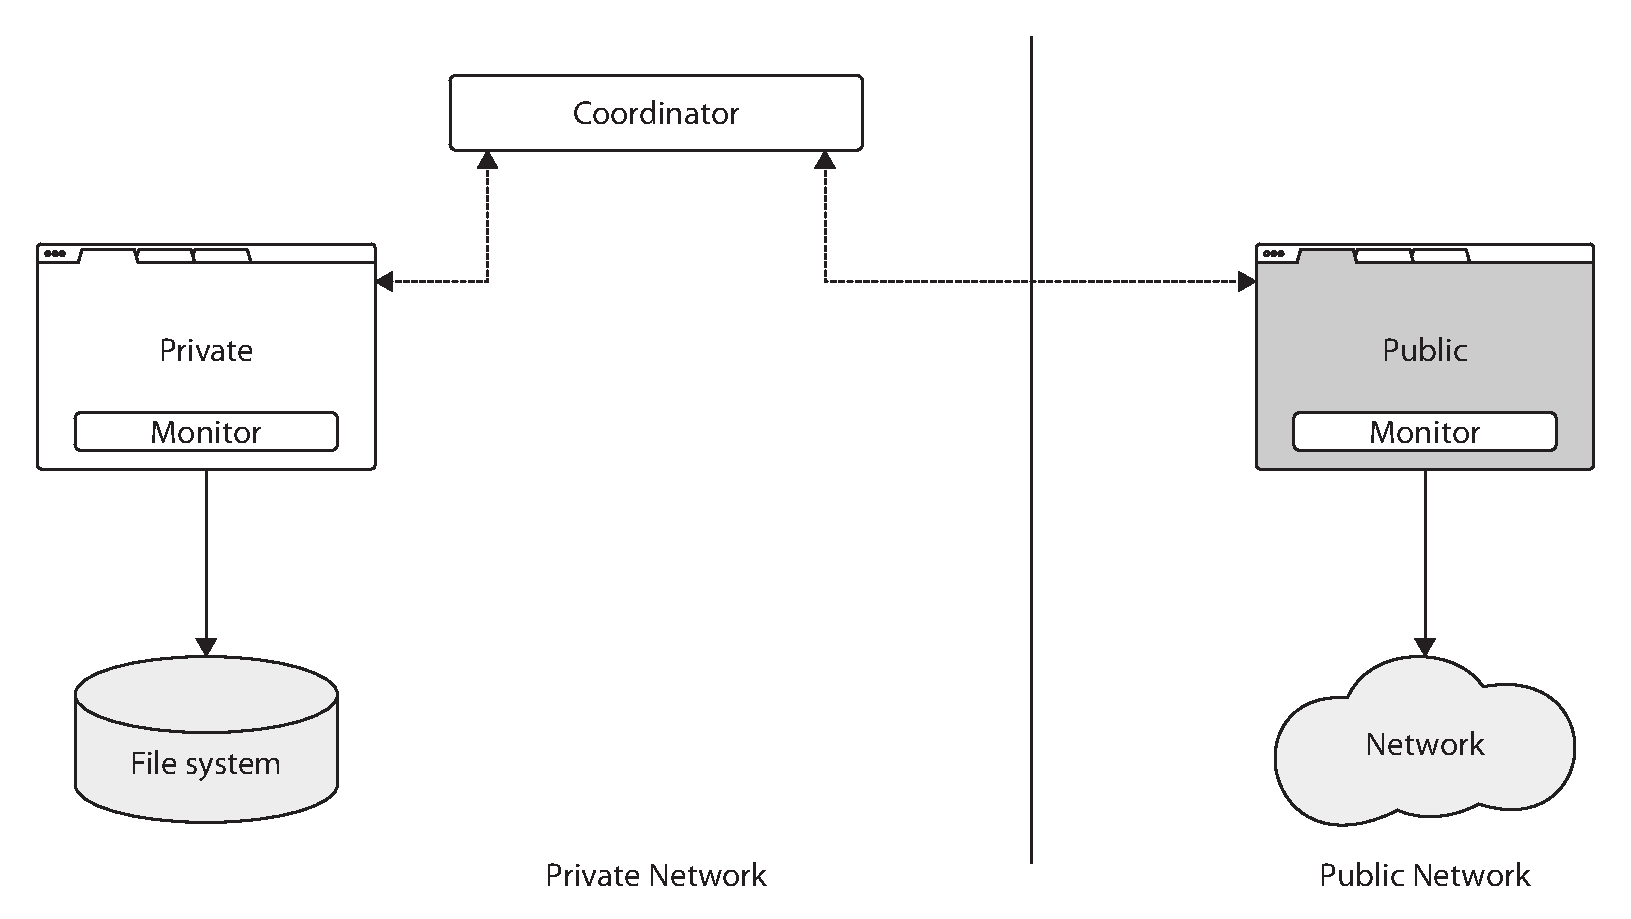
\includegraphics[width=0.75\columnwidth]{applications/figures/honeypot}
    \caption{The architecture of the multi-variant honeypot system.}
    \label{fig:security-honeypot}
  \end{center}
\end{figure}

The architecture of our prototype system is depicted in
Figure~\ref{fig:security-honeypot}.  To enforce strong separation, in our
prototype, each variant can be run on a different machine. Even if attackers
manage to subvert our monitoring infrastructure and gain the full access to the
operating system, the impact of such intrusion can be minimal as the machine
which runs the public version will not contain any critical resources and will
be ideally running inside the demilitarized zone (DMZ) to prevent access to
other machines on the network.  Such architecture, however, precludes the use
of the shared ring buffer and the streaming architecture
(\S\ref{sec:streaming}). Instead, in our prototype, we use network sockets to
transfer events between variants and the monitor. This has a negative impact on
the performance; we have observed a per-system call overhead of
\numrange{18}{25}$\times$ in our microbenchmarks. However, we believe that in
the case of honeypot systems, performance overhead is not the most important
factor, unlike security guarantees, as the applications running on top of such
systems are not expected to be used in performance critical scenarios.

We have tested our prototype by running two variants of \lighttpd 1.4.28 on top
of our honeypot system, where the private variant has been compiled with all
the security provided by GCC enabled while the public variant did not use any
of these.
%\footnote{We used \lstinline`-fstack-protector-all -Wstack-protector --param
%ssp-buffer-size=4 -pie -PIE -ftrapv -D_FORTIFY_SOURCE=2 -z relro,now` GCC
%options for the private variant and \lstinline`-fno-stack-protector -z
%execstack` options for the the public variant.}
We then used an existing exploit~\cite{erickson:hacking-networking} to attack the public variant and
inject the shellcode,\footnote{\url{http://www.shell-storm.org/shellcode/files/shellcode-658.php}}
which tries to add a root user with a custom password to the system. This
attack has been successfully detected and prevented by the honeypot monitor.

\section{Future work}
\label{sec:future-work}

There are number of other ways in which both systems could be extended in the
future. In general, we would like to increase the flexibility, to expand the
range of versions we could run in parallel. This means both tolerance to a
wider set of changes as well as ability to detect different type of
divergences.

The recovery mechanism in \mx is based on the ability of restarting the crashed
version using a lightweight checkpointing mechanism. In our current
implementation, we only keep the latest checkpoint for performance reasons.
However, this means that \mx cannot recover a fault caused by a change past the
last checkpoint. We could raise this limitation by keeping more checkpoints and
iteratively retry them if we fail to recover using more recent one. There is a
trade-off involved: keeping more checkpoints incurs higher performance overhead
and we would also need to keep the log of all the system calls between the
checkpointed state and the point of failure, akin to \varan's record \& replay
mechanism.

While \varan allows execution of large number of versions in parallel, the
number of versions is currently set at start. We would like enhance our
prototype implementation with the ability to dynamically adjust the number of
versions that are run concurrently. This will ensure that multi-version
applications will be able to utilize all available resources (\ie idle
processor time) without affecting the overall system performance during peak
load.

While scaling down the number of versions is straightforward, to scale up we
would an ability to start new versions and allow them to catch up with the
leader. There are different ways in which such support could be implemented. For
applications structured around a central dispatch loop (\eg network servers or
applications with graphical user interface), we could infer the loop headers
(either statically~\cite{DJgraphs,havlak} or dynamically~\cite{sato11}) and
allow the new versions to "catch up" with the leader at the beginning of the
dispatch loop. The same mechanism could be also used to replace the failing
version in the transparent failover mode.

% Finally, we would like to be able to transparently run multi-version
% applications on multiple underlying platforms, ranging from
% multicore processors to large-scale data centers.  This requires the
% ability to span our virtualized environment across multiple logical as
% well as physical nodes.  In particular, we aim to include the
% possibility of executing certain versions of an application remotely,
% to enable scenarios with hundreds or even thousands of application
% versions.

% During execution, we perform regular checkpoints (\eg based on
% \textstt{fork} which uses copy-on-write internally) and we also record
% all the system calls since the last checkpoint.  On recovery, we first
% restore the failing version from the latest checkpoint and then replay
% all recorded system calls to bring the application to a state just
% before the crash.  The frequency of checkpointing involves a
% trade-off: frequent checkpointing incurs a performance overhead, but
% infrequent checkpointing requires more space to store the system call
% logs.  The two variants of MV execution discussed in this proposal
% would correspond to the two extremes: running the two versions in
% parallel and synchronising the execution at every system call
% (parallel MV execution), and executing the two versions sequentially
% with the second version only being run when the first version crashes
% (sequential MV execution).

% With checkpointing, we can explore points in-between the two extremes,
% and control the different trade-offs more precisely by adaptively
% changing the frequency with which the checkpoints are taken.  One
% strategy would be to monitor the rate of system calls issued by an
% application and adapt the checkpointing rate accordingly.  Ideally, one
% would checkpoint frequently enough to have the log fit in memory, which
% could significantly reduce the recording overhead by eliminating
% expensive I/O operations.

% Furthermore, the way we employ the record and replay mechanism gives us
% additional control over the recovery process.  We can only start replaying the
% execution after the version being recorded crashes, or we can reduce the
% recovery time by running both versions in parallel, recording system calls to a
% log in one version and immediately replaying them in the second version (which
% potentially could be run at lower priority).  While the former variant has been
% used in other contexts, the latter one is novel and more suitable for
% multi-version execution.  Furthermore, by restricting the maximal/minimal
% length of the system call log we can explore the design space in-between these
% two variants.

